\section{FLiDASH: Federated Adaptive Bitrate Live Streaming over Locality Sensitive Playback Coalitions}
\red{Live streaming is a unique service in the Internet which is alternative to TV broadcast yet more flexible. Few live streaming provider allow ability add custom delay. However, most popular flavor of live streaming is without any user defined delays. The live stream have a unique property of synchronous playback by millions of players. In case of mega event, we find another interesting property that many player belongs same local networks. There is two special case exists a) Internet on cable where users have different connection even though they are connected via local networks, b) shared Internet connection where multiple user/player share same Internet backbone. We want to develop a DASH based live streaming system where players forms coalition if they are connected via local network and stream the live video as a group. Incase of large network, Application-Layer Traffic Optimization (ALTO) server will be use to find appropriate players. Our goal is to improve quality for entire coalition and every player have to contribute towards the common goal.}
\subsection{Architecture}
Unlike DASH streaming system, FLiDASH system have three components, these are a) streaming server: host the the video data, b) streaming client: plays the video, c) proximity server: identify nearby player. While the streaming server is unmodified webserver, the client is designed specially for live video streaming. It act as normal DASH based player if there is no other players nearby. However, if continuously look for nearby player to form coalition. As broadcast is confine to broadcast domain only, we use proximity server to find near by players. Before quality formation, clients first whether they compatible or not primarily by expected quality level. Once coalition is formed, coalition based video streaming system starts.
\subsection{Adaptive streaming system}
As FLiDASH is a collaborative streaming system, we need to decide which player going to download which segment and what will be the quality. Here we call a player is busy if it is downloading a segment from the CDN otherwise it is idle. Our aim to maximize quality by keeping every player busy all the time. We achieve this goal by scheduling segment to a player which is idle for maximum time or who have least amount to be downloaded. Once player is chosen, that player is informed to download the segment and respected player decide the segment quality based on the its bandwidth, deadline to finish downloading and other players decision. We have introduce a fail safe mechanism in case designated player fails to download the segment before the deadline. More details are available in thesis.
\subsection{Evaluation}
We have performed evaluation on the simulated environment with two type of scenario a) every players have there own Internet connection and b) players share a common internet connection. We have developed a prototype using {\tt python} and evaluated our system. We compare our system with modern ABR algorithm BOLA, MPC and Pensieve and a system with Distributed Hash Table (DHT). We compare the QoE of both the scenario in the Fig.~\ref{fig:FLiDASH:QoE} which supports our claim that collaboration improve the over all quality.
\begin{figure}[h]
	\captionsetup[subfigure]{width=0.49\linewidth}
	\begin{center}
		\subfloat[\label{fig:FLiDASH:ind_qoe}Indipendent Internet connection]{
			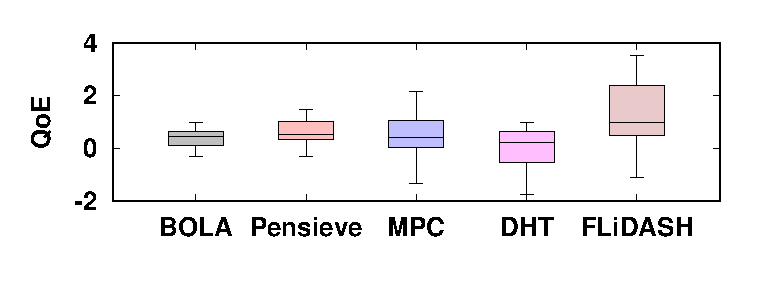
\includegraphics[width=0.49\linewidth]{img/FLiDASH/ind_qoe_box_1}
		}
		\subfloat[\label{fig:FLiDASH:shared_qoe}Shared Internet connection]{
			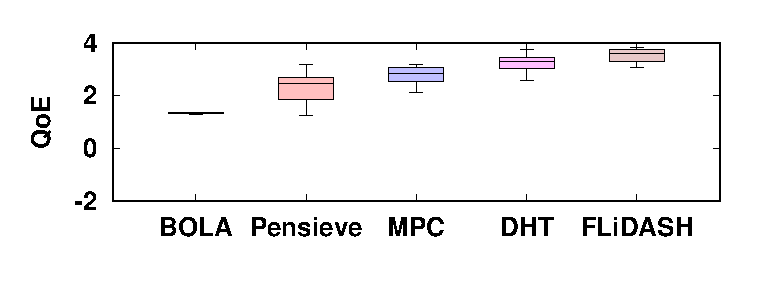
\includegraphics[width=0.49\linewidth]{img/FLiDASH/shared_qoe_box_1}
		}
	\end{center}
	\caption{\label{fig:FLiDASH:QoE}Comparison of video streaming system in terms of QoE}
\end{figure}
